\documentclass[10pt,twocolumn,letterpaper]{article}

% --- Page Geometry matching ICML / Top-Tier ML & Systems Conferences ---
\usepackage[
  letterpaper,
  top=1.0in,
  bottom=1.0in,
  left=0.875in,
  right=0.875in,
  columnsep=0.25in
]{geometry}

% --- Typography: Times Roman + Microtypography ---
\usepackage{times}
\usepackage{mathptmx}
\usepackage{microtype}
\usepackage[utf8]{inputenc}
\usepackage[T1]{fontenc}

% --- Mathematics & Theorems ---
\usepackage{amsmath,amsfonts,amssymb,amsthm}
\newtheorem{theorem}{Theorem}
\newtheorem{lemma}[theorem]{Lemma}
\newtheorem{definition}[theorem]{Definition}
\newtheorem{corollary}[theorem]{Corollary}

% --- Professional Graphics & Tables ---
\usepackage{graphicx}
\usepackage{booktabs}
\usepackage{array}
\usepackage{url}
\usepackage{cite}
\usepackage{textcomp}
\usepackage{tikz}
\usetikzlibrary{arrows,arrows.meta,positioning,shapes.geometric,calc,fit}

% --- Running Headers & Footers (ICML style) ---
\usepackage{fancyhdr}
\pagestyle{fancy}
\fancyhf{}
\fancyhead[C]{\small\itshape Architectural Foundations of Relational Subqueries, Quantified Predicates, and Virtual Views}
\fancyfoot[C]{\small\thepage}
\renewcommand{\headrulewidth}{0.4pt}
\renewcommand{\footrulewidth}{0pt}

% Suppress header on first page
\fancypagestyle{firstpage}{
  \fancyhf{}
  \fancyfoot[L]{\footnotesize\itshape Proceedings of Industrial \& Systems Database Architecture, 2026.}
  \fancyfoot[C]{\small\thepage}
  \renewcommand{\headrulewidth}{0pt}
}

% --- Compact Section Titles (ICML style: 1. Introduction, 1.1. Subheading) ---
\usepackage{titlesec}
\titleformat{\section}{\large\bfseries}{\thesection.}{0.5em}{}
\titleformat{\subsection}{\normalsize\bfseries}{\thesubsection.}{0.5em}{}
\titleformat{\subsubsection}{\small\bfseries}{\thesubsubsection.}{0.5em}{}
\titlespacing*{\section}{0pt}{1.5ex plus 0.5ex minus 0.2ex}{1.0ex plus 0.2ex}
\titlespacing*{\subsection}{0pt}{1.2ex plus 0.4ex minus 0.2ex}{0.8ex plus 0.2ex}
\titlespacing*{\subsubsection}{0pt}{1.0ex plus 0.3ex minus 0.2ex}{0.6ex plus 0.2ex}

% --- Listings Formatting for SQL & Code ---
\usepackage{listings}
\usepackage{xcolor}

\definecolor{codeblue}{rgb}{0.0,0.2,0.7}
\definecolor{codegreen}{rgb}{0,0.5,0}
\definecolor{codegray}{rgb}{0.4,0.4,0.4}
\definecolor{codepurple}{rgb}{0.5,0,0.7}
\definecolor{backcolour}{rgb}{0.98,0.98,0.98}

\lstdefinestyle{sqlStyle}{
    backgroundcolor=\color{backcolour},   
    commentstyle=\color{codegreen}\itshape,
    keywordstyle=\color{codeblue}\bfseries,
    numberstyle=\tiny\color{codegray},
    stringstyle=\color{codepurple},
    basicstyle=\ttfamily\scriptsize,
    breakatwhitespace=false,         
    breaklines=true,                 
    captionpos=b,                    
    keepspaces=true,                 
    numbers=none,
    showspaces=false,                
    showstringspaces=false,
    showtabs=false,                  
    tabsize=2,
    frame=single,
    rulecolor=\color{black!20}
}
\lstset{style=sqlStyle}

\begin{document}

\twocolumn[
  \begin{@twocolumnfalse}
    \begin{center}
      {\LARGE\bfseries Architectural Foundations of Relational Subqueries, Quantified Predicates, and Virtual Views: Modular Decomposition, Correlated Loop Complexity, NULL-Safe Existence Semantics, and AST Merge Mechanics in SQL Database Systems \par}
      \vspace{1.0em}
      {\large\bfseries Pavan Gopala \par}
      \vspace{0.3em}
      {\small Database Systems and Relational Architecture Group \par}
      {\small\texttt{pavan@enterprise-sql.org} \par}
      \vspace{1.5em}
    \end{center}
  \end{@twocolumnfalse}
]

\thispagestyle{firstpage}

\begin{center}
  {\bfseries\large Abstract}
\end{center}
\vspace{-0.5em}
{\small In relational database management systems (RDBMS), decomposing complex analytical questions into modular, verifiable expressions relies fundamentally on nested subqueries and relational view abstractions. Built on relational calculus and first-order logic, subqueries operationalize the divide-and-conquer paradigm across filtering (\texttt{WHERE}, \texttt{HAVING}), projection (\texttt{SELECT}), and transient relation derivation (\texttt{FROM}). This paper presents an exhaustive systems engineering investigation of relational subqueries, correlated execution dynamics, quantified comparison predicates, and virtual views derived from foundational relational theory and enterprise SQL engines (such as MySQL InnoDB). We formalize the cardinality constraints of scalar subqueries, contrasting deterministic singleton reductions against runtime Error 1242 violations. We dissect multi-row set membership (\texttt{IN}) and derived tables in the \texttt{FROM} clause, proving mathematically why derived tables require mandatory aliasing and how they resolve the ANSI SQL prohibition against nested aggregate functions (e.g., computing \texttt{MIN(AVG(psp))}). Furthermore, we formalize quantified comparison operators (\texttt{ALL} and \texttt{ANY}), establishing the semantic necessity of \texttt{ANY} for multi-row inequality evaluations and demonstrating the non-intuitive vacuous truth behavior of \texttt{ALL} over empty sets. We conduct rigorous computational complexity analyses contrasting decoupled independent subqueries against correlated subqueries, demonstrating how unnesting and decorrelation reduce execution latency from quadratic $\mathcal{O}(N \cdot M)$ tuple iterations to linear $\mathcal{O}(N + M)$ index lookups. Crucially, we prove the fundamental three-valued logic (3VL) divergence between \texttt{NOT IN} and \texttt{NOT EXISTS}, revealing how NULL values in subqueries catastrophically yield \texttt{UNKNOWN} and empty result sets under \texttt{NOT IN}, whereas \texttt{NOT EXISTS} guarantees complete NULL-immunity. Finally, we dissect the execution mechanics of relational views, contrasting AST expansion (\texttt{ALGORITHM = MERGE}) with internal materialization (\texttt{TEMPTABLE}), and establish the relational invariants governing view updatability. All principles are substantiated by vector TikZ architectural diagrams, relational truth tables, formal complexity proofs, and production SQL implementations.}

\vspace{1.0em}
\noindent\textbf{Keywords:} Relational Databases, Subqueries, Correlated Subqueries, Quantified Predicates, ALL and ANY, EXISTS, Three-Valued Logic, Virtual Views, Query Optimization, MySQL InnoDB.
\vspace{1.2em}

\section{Introduction}
\label{sec:intro}

In modern enterprise computing architectures, Relational Database Management Systems (RDBMS) such as MySQL InnoDB, PostgreSQL, and Oracle are tasked with executing complex analytical and transactional queries over highly normalized relational schemas. While elementary queries retrieve or filter data from single tables, enterprise decision systems frequently require multi-stage relational reasoning: identifying entities that exceed dynamically calculated population thresholds, verifying referential memberships across distinct role hierarchies, computing non-nestable aggregate summaries, and establishing access-controlled data abstractions.

To resolve complex relational inquiries declaratively, SQL provides the **Subquery** mechanism. Formalized within relational calculus and first-order predicate logic \cite{codd1970, date2004}, a subquery (or nested query) is an auxiliary \texttt{SELECT} statement encapsulated within an enclosing parent query block. Subqueries embody the classical algorithmic principle of **Divide and Conquer**: decomposing a monolithic relational problem into modular, verifiable subproblems whose intermediate results feed directly into upstream evaluation operators.

\begin{figure*}[htbp]
\centering
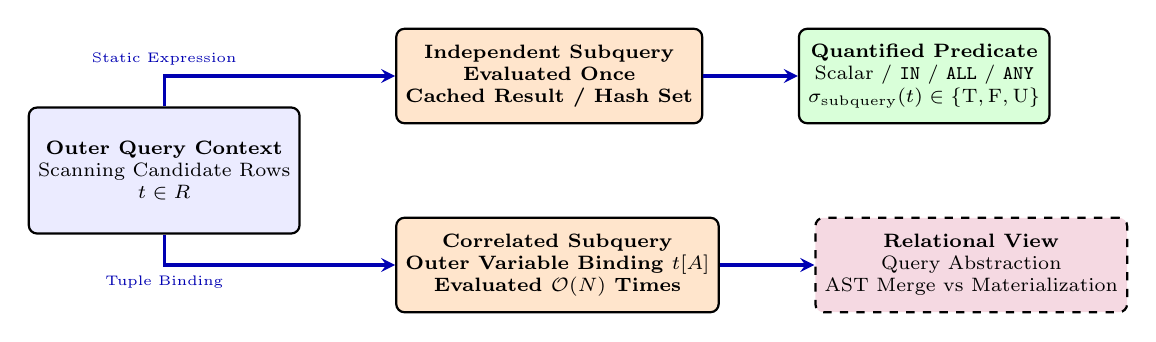
\begin{tikzpicture}[
    node distance=0.8cm and 0.8cm,
    parentbox/.style={draw, rectangle, rounded corners=3pt, thick, align=center, fill=blue!8, minimum width=3.2cm, minimum height=1.6cm, font=\scriptsize},
    subbox/.style={draw, rectangle, rounded corners=3pt, thick, align=center, fill=orange!20, minimum width=3.0cm, minimum height=1.2cm, font=\scriptsize\bfseries},
    proc/.style={draw, rectangle, rounded corners=3pt, thick, align=center, fill=green!15, minimum width=2.6cm, minimum height=1.2cm, font=\scriptsize},
    viewbox/.style={draw, rectangle, rounded corners=3pt, dashed, thick, align=center, fill=purple!15, minimum width=3.0cm, minimum height=1.2cm, font=\scriptsize},
    arr/.style={->, >=stealth, very thick, color=blue!70!black}
]
    \node[parentbox] (outer) {\textbf{Outer Query Context}\\Scanning Candidate Rows\\$t \in R$};
    \node[subbox, right=1.2cm of outer, yshift=1.2cm] (uncorr) {\textbf{Independent Subquery}\\Evaluated Once\\Cached Result / Hash Set};
    \node[subbox, right=1.2cm of outer, yshift=-1.2cm] (corr) {\textbf{Correlated Subquery}\\Outer Variable Binding $t[A]$\\Evaluated $\mathcal{O}(N)$ Times};
    \node[proc, right=1.2cm of uncorr] (pred) {\textbf{Quantified Predicate}\\Scalar / \texttt{IN} / \texttt{ALL} / \texttt{ANY}\\$\sigma_{\text{subquery}}(t) \in \{\text{T}, \text{F}, \text{U}\}$};
    \node[viewbox, right=1.2cm of corr] (views) {\textbf{Relational View}\\Query Abstraction\\AST Merge vs Materialization};
    
    \draw[arr] (outer) |- node[above, font=\tiny] {Static Expression} (uncorr);
    \draw[arr] (outer) |- node[below, font=\tiny] {Tuple Binding} (corr);
    \draw[arr] (uncorr) -- (pred);
    \draw[arr] (corr) -- (views);
\end{tikzpicture}
\caption{The Architectural Taxonomy of Relational Subqueries and Virtual Views. Subqueries decompose parent relational operations into independent cached evaluations or tuple-correlated iterations, while relational views encapsulate multi-stage logic into reusable schema abstractions.}
\label{fig:taxonomy}
\end{figure*}

Subqueries operate across multiple structural clauses of SQL:
\begin{enumerate}
    \item \textbf{Filtering Clauses (\texttt{WHERE} and \texttt{HAVING})}: Enforcing scalar comparisons ($=, <, >$), set-membership evaluations (\texttt{IN}), quantified relational bounds (\texttt{ALL}, \texttt{ANY}), and existential verifications (\texttt{EXISTS}).
    \item \textbf{Table-Expression Clauses (\texttt{FROM})}: Constructing transient derived relations that bypass SQL's prohibition against nested aggregate functions.
    \item \textbf{Projection Clauses (\texttt{SELECT})}: Computing scalar dimensional mappings dynamically for each output row.
\end{enumerate}

Based on pedagogical and industrial database engineering curriculum notes (specifically \cite{sql6notes}), this research paper presents an exhaustive architectural analysis of relational subqueries, correlated query processing, quantified comparison predicates, and virtual relational views. We formalize the algebraic mechanics of scalar, columnar, and table subqueries, analyze the computational complexity trade-offs of subquery correlation ($\mathcal{O}(N + M)$ vs. $\mathcal{O}(N \cdot M)$), prove the mathematical and NULL-handling divergence between \texttt{IN} and \texttt{EXISTS}, and examine the physical execution of virtual views under MySQL InnoDB.

% -----------------------------------------------------------------------------
\section{Scalar Subqueries and Cardinality Enforcement}
\label{sec:scalar_subqueries}

The most elementary class of nested query is the **Scalar Subquery**, which produces an output relation consisting of exactly one row and one column ($1 \times 1$).

\subsection{Syntax and Operational Mechanics}
Consider the canonical \texttt{students} relation from \cite{sql6notes}, structured with attributes \texttt{id}, \texttt{name}, \texttt{batch\_id}, and \texttt{psp} (problem-solving percentage). Suppose business logic requires identifying all students who performed strictly better than a specific individual (e.g., student with \texttt{id = 2}, named Rohit with \texttt{psp = 90}):

\begin{lstlisting}[language=SQL]
SELECT id, name, batch_id, psp
FROM students
WHERE psp > (
    SELECT psp 
    FROM students 
    WHERE id = 2
);
\end{lstlisting}

The execution engine processes this statement in two distinct phases:
\begin{enumerate}
    \item \textbf{Inner Scalar Evaluation}: The subquery \texttt{SELECT psp FROM students WHERE id = 2} executes against the primary key index, locating Rohit's record and extracting the scalar value $90$.
    \item \textbf{Outer Selection Execution}: The scalar literal $90$ replaces the subquery expression in the outer Abstract Syntax Tree (AST). The outer query evaluates \texttt{WHERE psp > 90}, emitting only student Sachin (\texttt{id = 7}, \texttt{psp = 95}).
\end{enumerate}

\subsection{Cardinality Invariants and Runtime Violations}
Standard relational comparison operators ($=, !=, <, <=, >, >=$) are strictly binary operations defined over scalar operands:
\begin{equation}
\text{op}: D \times D \longrightarrow \{\text{TRUE}, \text{FALSE}, \text{UNKNOWN}\}
\end{equation}

If an inner subquery evaluated within a scalar comparison operator returns more than one tuple:
\begin{lstlisting}[language=SQL]
-- RUNTIME CARDINALITY VIOLATION:
SELECT * FROM students
WHERE psp > (SELECT psp FROM students WHERE batch_id = 1);
\end{lstlisting}
Because \texttt{batch\_id = 1} contains multiple students (Virat with \texttt{psp = 80} and Rohit with \texttt{psp = 90}), the inner query returns a multi-row column vector $\{80, 90\}$. The execution engine cannot evaluate whether a candidate score is greater than an entire set without explicit quantification, aborting execution with MySQL Error 1242:
\begin{lstlisting}[basicstyle=\ttfamily\scriptsize]
ERROR 1242 (21000): Subquery returns more than 1 row
\end{lstlisting}

\subsubsection{Defensive Production Engineering Patterns}
To guarantee that subqueries evaluated within scalar operators never trigger runtime cardinality exceptions, software engineers deploy two defensive patterns:
\begin{itemize}
    \item \textbf{Deterministic Scalar Aggregators}: Wrapping the inner projection in an aggregate function (such as \texttt{MAX(psp)} or \texttt{MIN(psp)}), guaranteeing that regardless of row volume, exactly one scalar is emitted.
    \item \textbf{Bounded Deterministic Windowing}: Appending an explicit sort and limit directive: \texttt{ORDER BY psp DESC LIMIT 1}.
\end{itemize}

% -----------------------------------------------------------------------------
\section{Set-Membership Subqueries: The IN Clause and Semi-Joins}
\label{sec:in_subqueries}

When a subquery returns multiple rows along a single attribute column (a 1D column vector of dimension $m \times 1$), standard scalar comparison operators fail. In such scenarios, set-membership operators, primarily \texttt{IN}, are deployed.

\subsection{Problem Formulation: Identifying Dual-Role Entities}
Consider an operational table where individuals hold dual classifications: students who also serve as Teaching Assistants (\texttt{is\_ta = 1}):
\begin{lstlisting}[language=SQL]
-- Table Schema
CREATE TABLE students (
    id INT PRIMARY KEY,
    name VARCHAR(50),
    is_student TINYINT(1) DEFAULT 1,
    is_ta TINYINT(1) DEFAULT 0
);
\end{lstlisting}

Requirement: \textit{``Find the student IDs of all individuals whose name matches the name of any Teaching Assistant.''}

This query is formulated via an \texttt{IN} subquery:
\begin{lstlisting}[language=SQL]
SELECT id, name
FROM students
WHERE name IN (
    SELECT name 
    FROM students 
    WHERE is_ta = 1
);
\end{lstlisting}

\begin{definition}[Set-Membership Subquery Semantics]
Let $R$ be the outer relation and $S_{\text{sub}}$ be the set of values emitted by the inner query:
\begin{equation}
S_{\text{sub}} = \{ t_{\text{inner}}[A] \mid t_{\text{inner}} \in S \land p(t_{\text{inner}}) = \text{TRUE} \}
\end{equation}
A candidate outer tuple $t_{\text{outer}} \in R$ is retained if and only if:
\begin{equation}
t_{\text{outer}}[A] \in S_{\text{sub}} \iff \exists s \in S_{\text{sub}} \text{ such that } t_{\text{outer}}[A] = s
\end{equation}
\end{definition}

In the pedagogical dataset from \cite{sql6notes}:
\begin{itemize}
    \item TAs are Virat (\texttt{id = 1}), Hardik (\texttt{id = 4}), and Rohit (\texttt{id = 6}).
    \item The inner query emits $S_{\text{sub}} = \{\text{'Virat'}, \text{'Hardik'}, \text{'Rohit'}\}$.
    \item In the outer query, student Rohit (\texttt{id = 2}, who is not a TA) is correctly captured alongside \texttt{id = 1, 4, 6} because his name matches an element in $S_{\text{sub}}$. The query returns IDs: $\{1, 2, 4, 6\}$.
\end{itemize}

\begin{table*}[htbp]
\caption{Comparative Dimensionality and Syntactic Clauses of Relational Subqueries}
\label{tab:dimensionality}
\centering
\scriptsize
\begin{tabular}{p{2.6cm}p{2.2cm}p{2.4cm}p{3.2cm}p{4.6cm}}
\toprule
\textbf{Subquery Class} & \textbf{Output Geometry} & \textbf{Permissible Clauses} & \textbf{Evaluation Operators} & \textbf{Optimizer Execution Strategy} \\
\midrule
\textbf{Scalar Subquery} & Single Value ($1 \times 1$) & \texttt{SELECT}, \texttt{WHERE}, \texttt{HAVING} & Scalar comparisons ($=, <, >, \le, \ge$) & Evaluated once; value cached into AST literal. \\
\textbf{Columnar Subquery} & Single Column ($m \times 1$) & \texttt{WHERE}, \texttt{HAVING} & \texttt{IN}, \texttt{NOT IN}, \texttt{ANY}, \texttt{ALL} & Semi-join materialization or temporary hash set lookup. \\
\textbf{Row Subquery} & Single Row ($1 \times k$) & \texttt{WHERE}, \texttt{HAVING} & Tuple equality: $(a, b) = (\text{subquery})$ & Evaluated once; tuple unpacked into scalar registers. \\
\textbf{Table Subquery} & Multi-Row, Multi-Col ($m \times k$) & \texttt{FROM}, \texttt{JOIN} & Relational scans, explicit aliasing & Derived table merging or on-disk/in-memory temporary table. \\
\bottomrule
\end{tabular}
\end{table*}

\subsection{Query Optimizer Semi-Join Transformations}
In naive relational engines, an \texttt{IN} subquery was executed as a nested loop: for every outer row, the inner subquery was re-evaluated, resulting in $\mathcal{O}(N \cdot M)$ complexity.

Modern query optimizers (including MySQL 8.0+) transform \texttt{WHERE col IN (SELECT ...)} into an optimized **Semi-Join**:
\begin{equation}
R \ltimes S = \{ r \in R \mid \exists s \in S \text{ such that } r.A = s.A \}
\end{equation}
Unlike an Inner Join (which duplicates outer rows if multiple inner rows match), a Semi-Join emits an outer row at most once, immediately terminating inner row scans upon the first referential match.

The optimizer selects among four primary semi-join execution strategies:
\begin{enumerate}
    \item \textbf{Materialization}: The inner query is evaluated once, deduplicated, and stored in an in-memory hash table. Outer rows probe the hash table in $\mathcal{O}(1)$ time.
    \item \textbf{FirstMatch}: The outer table drives a B+ Tree index seek into the inner table, halting immediately when the first match is confirmed.
    \item \textbf{LooseScan}: The inner table index is scanned using grouping skip-scans, emitting distinct values to join against the outer table.
    \item \textbf{Duplicate Weedout}: The tables are joined via standard inner join, and a temporary bitmap table removes duplicate outer row IDs.
\end{enumerate}

% -----------------------------------------------------------------------------
\section{Derived Tables in the FROM Clause and Non-Nesting Invariants}
\label{sec:derived_tables}

When a subquery appears in the \texttt{FROM} clause of a parent statement, it is formally termed a **Derived Table** (or inline view).

\subsection{The Mandatory Alias Invariant}
In ANSI SQL and MySQL, derived tables operate as anonymous relational expressions. Because every relation within the \texttt{FROM} clause must possess a resolvable namespace in the query data dictionary:
\begin{center}
\textbf{Every derived table in the \texttt{FROM} clause MUST be assigned an explicit table alias.}
\end{center}
Omitting an alias triggers MySQL Error 1248:
\begin{lstlisting}[basicstyle=\ttfamily\scriptsize]
ERROR 1248 (42000): Every derived table must have its own alias
\end{lstlisting}

\subsection{The Non-Nesting Aggregate Invariant}
A core syntactic and operational constraint of ANSI SQL is the strict prohibition of nested aggregate functions:
\begin{center}
\textbf{Expressions of the form \texttt{MIN(AVG(col))} or \texttt{SUM(COUNT(col))} are strictly illegal in SQL.}
\end{center}

Why are nested aggregates disallowed? An aggregate function collapses a multi-set of rows into a single scalar summary per group. At the time an aggregate executes within a query block, the input rows have already been collapsed; there is no secondary grouping context within the same logical lifecycle phase to evaluate an outer aggregate.

\begin{figure*}[htbp]
\centering
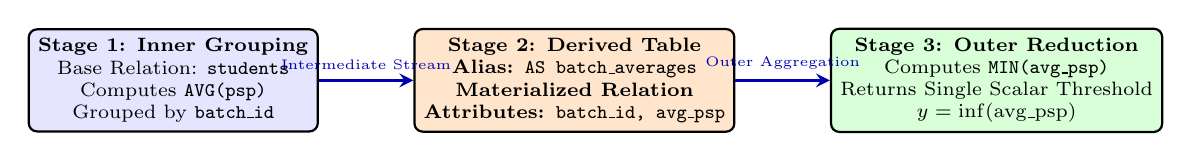
\begin{tikzpicture}[
    box/.style={draw, rectangle, rounded corners=3pt, thick, align=center, fill=blue!10, minimum width=2.8cm, minimum height=1.1cm, font=\scriptsize},
    dtbox/.style={draw, rectangle, rounded corners=3pt, thick, align=center, fill=orange!20, minimum width=3.4cm, minimum height=1.3cm, font=\scriptsize\bfseries},
    proc/.style={draw, rectangle, rounded corners=3pt, thick, align=center, fill=green!15, minimum width=2.8cm, minimum height=1.1cm, font=\scriptsize},
    arr/.style={->, >=stealth, very thick, color=blue!70!black}
]
    \node[box] (inner) {\textbf{Stage 1: Inner Grouping}\\Base Relation: \texttt{students}\\Computes \texttt{AVG(psp)}\\Grouped by \texttt{batch\_id}};
    \node[dtbox, right=1.2cm of inner] (dt) {\textbf{Stage 2: Derived Table}\\Alias: \texttt{AS batch\_averages}\\Materialized Relation\\Attributes: \texttt{batch\_id, avg\_psp}};
    \node[proc, right=1.2cm of dt] (outer) {\textbf{Stage 3: Outer Reduction}\\Computes \texttt{MIN(avg\_psp)}\\Returns Single Scalar Threshold\\$y = \inf(\text{avg\_psp})$};
    
    \draw[arr] (inner) -- node[above, font=\tiny] {Intermediate Stream} (dt);
    \draw[arr] (dt) -- node[above, font=\tiny] {Outer Aggregation} (outer);
\end{tikzpicture}
\caption{Derived Table Resolution for Multi-Stage Aggregation. SQL's prohibition against nested aggregates (\texttt{MIN(AVG())}) is resolved by materializing the first-stage group averages into a derived table (\texttt{batch\_averages}) upon which the second-stage outer reduction operates.}
\label{fig:derived_table}
\end{figure*}

\subsection{Multi-Stage Aggregation via Derived Tables}
Consider the challenging multi-stage problem from \cite{sql6notes}:
\begin{center}
\textit{``Find the data of all students whose PSP is strictly greater than the minimum batch average PSP across the entire academy.''}
\end{center}

Because \texttt{MIN(AVG(psp))} is forbidden, this query requires a three-stage relational decomposition:
\begin{enumerate}
    \item \textbf{Stage 1 (Inner Grouping)}: Compute the average PSP for each batch:
    \begin{lstlisting}[language=SQL]
    SELECT avg(psp) AS avg_psp 
    FROM students 
    GROUP BY batch_id;
    \end{lstlisting}
    \item \textbf{Stage 2 (Derived Table Reduction)}: Calculate the minimum of those batch averages by querying the materialized derived table:
    \begin{lstlisting}[language=SQL]
    SELECT min(avg_psp) 
    FROM (
        SELECT avg(psp) AS avg_psp 
        FROM students 
        GROUP BY batch_id
    ) AS batch_averages;
    \end{lstlisting}
    \item \textbf{Stage 3 (Outer Selection)}: Filter individual students whose personal PSP exceeds this dynamically computed threshold:
    \begin{lstlisting}[language=SQL]
    SELECT * FROM students
    WHERE psp > (
        SELECT min(avg_psp) 
        FROM (
            SELECT avg(psp) AS avg_psp 
            FROM students 
            GROUP BY batch_id
        ) AS batch_averages
    );
    \end{lstlisting}
\end{enumerate}

As illustrated in Figure~\ref{fig:derived_table}, derived tables enable multi-pass analytical reductions while maintaining strict compliance with relational algebra invariants.

% -----------------------------------------------------------------------------
\section{Quantified Comparison Predicates: ALL and ANY}
\label{sec:quantified_predicates}

When comparing a scalar attribute against a set of values emitted by a columnar subquery using relational inequalities ($<, \le, >, \ge$), SQL provides **Quantified Comparison Predicates**: \texttt{ALL} and \texttt{ANY} (synonymous with \texttt{SOME}).

\subsection{Mathematical Formalization}
Let $x$ be a scalar attribute value and $S = \{s_1, s_2, \dots, s_m\}$ be a non-empty set of values returned by a subquery:
\begin{align}
x > \text{ALL}(S) &\iff \forall s \in S, \; x > s \iff x > \max(S) \\
x < \text{ALL}(S) &\iff \forall s \in S, \; x < s \iff x < \min(S) \\
x > \text{ANY}(S) &\iff \exists s \in S, \; x > s \iff x > \min(S) \\
x < \text{ANY}(S) &\iff \exists s \in S, \; x < s \iff x < \max(S) \\
x = \text{ANY}(S) &\iff \exists s \in S, \; x = s \iff x \in S \iff x \text{ IN } S
\end{align}

\subsection{Why ANY is Necessary: The Limitation of IN}
A common misconception among database developers is attempting to use \texttt{IN} with inequality comparisons:
\begin{lstlisting}[language=SQL]
-- SYNTAX ERROR: IN only supports equality!
SELECT * FROM students WHERE psp > IN (SELECT ...);
\end{lstlisting}
The \texttt{IN} predicate is mathematically restricted to set equality ($\in$). To express an inequality comparison against an arbitrary set, the query **must** employ \texttt{ANY} or \texttt{ALL}:
\begin{lstlisting}[language=SQL]
-- Correct formulation:
SELECT * FROM students WHERE psp > ANY (SELECT ...);
\end{lstlisting}

\subsection{Pedagogical Analysis of ALL and ANY}
Consider the domain examples from \cite{sql6notes}:
\begin{itemize}
    \item \textbf{Universal Bound (\texttt{ALL})}: \textit{``Virat has scored more than all other players.''}
    Virat's score ($80$) is compared against $\{90, 78, 89, 70, 78, 95\}$. Because $80 < 90$ and $80 < 95$, the universal condition fails ($\text{FALSE}$).
    \item \textbf{Existential Bound (\texttt{ANY})}: \textit{``Virat has scored more than any of the other players.''}
    Because Virat's score ($80$) exceeds at least one player (e.g., Kuldeep with $70$, Bumrah with $78$), the existential condition holds ($\text{TRUE}$).
\end{itemize}

\subsubsection{Industrial Query Formulations}
\begin{lstlisting}[language=SQL]
-- 1. Students whose PSP >= minimum PSP of EVERY batch:
SELECT * FROM students
WHERE psp >= ALL (
    SELECT min(psp) 
    FROM students 
    GROUP BY batch_id
);

-- 2. Students whose PSP > minimum PSP of AT LEAST ONE batch:
SELECT * FROM students
WHERE psp > ANY (
    SELECT min(psp) 
    FROM students 
    GROUP BY batch_id
);
\end{lstlisting}

\begin{table*}[htbp]
\caption{Complete Truth and Operational Semantics of Quantified Comparison Predicates}
\label{tab:quantified_truth}
\centering
\scriptsize
\begin{tabular}{p{2.6cm}p{3.2cm}p{3.0cm}p{3.0cm}p{3.2cm}}
\toprule
\textbf{Predicate Expression} & \textbf{Equivalent Scalar Formulation} & \textbf{Truth Condition} & \textbf{Empty Set Result ($S = \emptyset$)} & \textbf{NULL Contamination Hazard} \\
\midrule
$x > \text{ALL}(S)$ & $x > \max(S)$ & True iff $x > s$ for every $s \in S$ & \textbf{TRUE} (Vacuous Truth) & If any $s = \text{NULL}$ and $x \le \max$, yields \texttt{UNKNOWN}. \\
$x < \text{ALL}(S)$ & $x < \min(S)$ & True iff $x < s$ for every $s \in S$ & \textbf{TRUE} (Vacuous Truth) & If any $s = \text{NULL}$ and $x \ge \min$, yields \texttt{UNKNOWN}. \\
$x = \text{ALL}(S)$ & $x = s_1 \land |S| = 1$ & True iff all elements equal $x$ & \textbf{TRUE} (Vacuous Truth) & Yields \texttt{UNKNOWN} if any element is \texttt{NULL}. \\
\midrule
$x > \text{ANY}(S)$ & $x > \min(S)$ & True iff $x > s$ for at least one $s$ & \textbf{FALSE} & If no element satisfies $x > s$ and \texttt{NULL} exists $\to$ \texttt{UNKNOWN}. \\
$x < \text{ANY}(S)$ & $x < \max(S)$ & True iff $x < s$ for at least one $s$ & \textbf{FALSE} & If no element satisfies $x < s$ and \texttt{NULL} exists $\to$ \texttt{UNKNOWN}. \\
$x = \text{ANY}(S)$ & $x \text{ IN } S$ & True iff $x$ equals at least one $s$ & \textbf{FALSE} & If $x \notin S$ and \texttt{NULL} exists $\to$ \texttt{UNKNOWN}. \\
\bottomrule
\end{tabular}
\end{table*}

\subsection{Vacuous Truth and Three-Valued Logic Hazards}
Table~\ref{tab:quantified_truth} exposes critical boundary conditions in SQL quantified comparisons:
\begin{enumerate}
    \item \textbf{Vacuous Truth over Empty Sets}: If the inner subquery produces zero rows ($S = \emptyset$), first-order logic dictates that universal statements are vacuously true:
    \begin{equation}
    x > \text{ALL}(\emptyset) \equiv \text{TRUE} \quad \text{for any value of } x
    \end{equation}
    Conversely, existential quantification over an empty set is always false:
    \begin{equation}
    x > \text{ANY}(\emptyset) \equiv \text{FALSE}
    \end{equation}
    \item \textbf{NULL Contamination in ALL}: If the set $S$ contains even a single \texttt{NULL} value, evaluating $x > \text{ALL}(S)$ can never return True unless $x > s$ holds for all known values and the unknown value cannot violate it. In practice, comparing against sets with nulls frequently yields \texttt{UNKNOWN}, causing \texttt{WHERE} clauses to silently discard qualifying records.
\end{enumerate}

% -----------------------------------------------------------------------------
\section{Correlated Subqueries and Computational Complexity}
\label{sec:correlated_subqueries}

An independent subquery evaluates once, detached from the outer query context. In contrast, a **Correlated Subquery** references attributes from the enclosing query block, creating an interdependent execution loop.

\subsection{Operational Definition and Dependency Binding}
\begin{definition}[Correlated Subquery]
A subquery $Q_{\text{inner}}$ is correlated with an enclosing query $Q_{\text{outer}}$ if the evaluation of $Q_{\text{inner}}$ requires parameter bindings $t_{\text{outer}}[A]$ from the active tuple of $Q_{\text{outer}}$:
\begin{equation}
Q_{\text{inner}} = Q_{\text{inner}}(t_{\text{outer}}[A])
\end{equation}
Because $Q_{\text{inner}}$ is parameterized by outer tuple attributes, it cannot be pre-computed as a static standalone relation.
\end{definition}

\subsection{Case Study: Cohort-Relative Thresholds}
Consider the classic enterprise query: \textit{``Find all students whose PSP is strictly greater than the average PSP of their own respective batch.''}

\begin{lstlisting}[language=SQL]
SELECT s1.id, s1.name, s1.batch_id, s1.psp
FROM students s1
WHERE s1.psp > (
    SELECT AVG(s2.psp)
    FROM students s2
    WHERE s2.batch_id = s1.batch_id -- Correlation Binding!
);
\end{lstlisting}

\begin{figure*}[htbp]
\centering
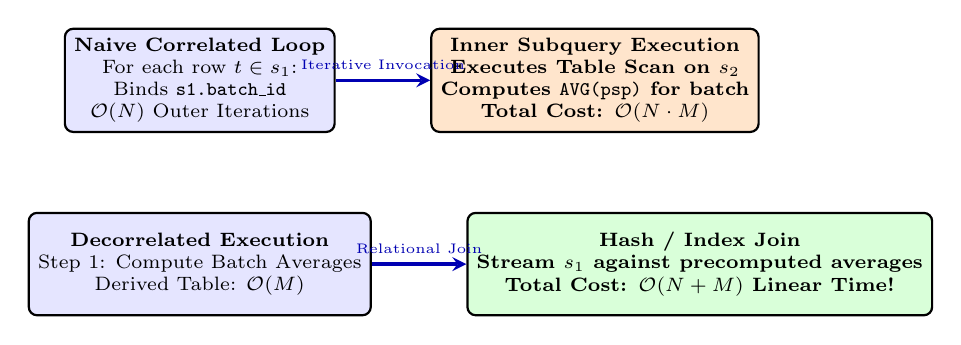
\begin{tikzpicture}[
    box/.style={draw, rectangle, rounded corners=3pt, thick, align=center, fill=blue!10, minimum width=3.2cm, minimum height=1.3cm, font=\scriptsize},
    corrbox/.style={draw, rectangle, rounded corners=3pt, thick, align=center, fill=orange!20, minimum width=3.4cm, minimum height=1.3cm, font=\scriptsize\bfseries},
    decorrbox/.style={draw, rectangle, rounded corners=3pt, thick, align=center, fill=green!15, minimum width=3.4cm, minimum height=1.3cm, font=\scriptsize\bfseries},
    arr/.style={->, >=stealth, very thick, color=blue!70!black}
]
    \node[box] (outer) {\textbf{Naive Correlated Loop}\\For each row $t \in s_1$:\\Binds \texttt{s1.batch\_id}\\$\mathcal{O}(N)$ Outer Iterations};
    \node[corrbox, right=1.2cm of outer] (inner) {\textbf{Inner Subquery Execution}\\Executes Table Scan on $s_2$\\Computes \texttt{AVG(psp)} for batch\\Total Cost: $\mathcal{O}(N \cdot M)$};
    
    \node[box, below=1.0cm of outer] (decorr_outer) {\textbf{Decorrelated Execution}\\Step 1: Compute Batch Averages\\Derived Table: $\mathcal{O}(M)$};
    \node[decorrbox, right=1.2cm of decorr_outer] (decorr_join) {\textbf{Hash / Index Join}\\Stream $s_1$ against precomputed averages\\Total Cost: $\mathcal{O}(N + M)$ Linear Time!};
    
    \draw[arr] (outer) -- node[above, font=\tiny] {Iterative Invocation} (inner);
    \draw[arr] (decorr_outer) -- node[above, font=\tiny] {Relational Join} (decorr_join);
\end{tikzpicture}
\caption{Correlated Execution Dynamics vs. Optimizer Subquery Decorrelation. Naive correlated execution incurs quadratic $\mathcal{O}(N \cdot M)$ nested loop latency. Modern optimizers decorrelate the query into a pre-aggregated hash join, reducing execution to linear $\mathcal{O}(N + M)$ time.}
\label{fig:decorrelation}
\end{figure*}

\subsection{Computational Complexity Trade-Offs}
In a naive execution engine, the procedural execution of this query behaves as a nested loop:
\begin{lstlisting}[language=SQL]
FOR each row s1 IN students DO:
    current_batch = s1.batch_id
    current_psp   = s1.psp
    
    -- Inner query re-executes for EVERY outer row:
    batch_avg = EXECUTE(
        SELECT AVG(psp) FROM students WHERE batch_id = current_batch
    )
    
    IF current_psp > batch_avg THEN:
        EMIT s1
\end{lstlisting}
\begin{theorem}[Correlated Subquery Nested Loop Complexity]
Let $N$ denote the cardinality of the outer relation and $M$ denote the cardinality of the inner relation. In the absence of index-assisted lookup or caching, unoptimized correlated subquery execution requires:
\begin{equation}
T_{\text{correlated}} = \mathcal{O}(N \cdot M)
\end{equation}
For a relation of $10^6$ rows, an unoptimized correlated subquery forces $10^{12}$ tuple comparisons, causing severe CPU thread locking and query timeouts.
\end{theorem}

\subsection{Optimizer Decorrelation and Subquery Unnesting}
To eliminate the quadratic performance penalty, modern query optimizers deploy **Subquery Decorrelation** (also termed Subquery Unnesting). The optimizer rewrites the correlated subquery into an explicit Inner Join against a pre-aggregated derived table:

\begin{lstlisting}[language=SQL]
-- Decorrelated Relational Equivalence Plan:
SELECT s.id, s.name, s.batch_id, s.psp
FROM students s
INNER JOIN (
    SELECT batch_id, AVG(psp) AS avg_batch_psp
    FROM students
    GROUP BY batch_id
) AS b_avg ON s.batch_id = b_avg.batch_id
WHERE s.psp > b_avg.avg_batch_psp;
\end{lstlisting}

As illustrated in Figure~\ref{fig:decorrelation}, the decorrelated query executes in linear $\mathcal{O}(N + M)$ time: the batch averages are computed once in a single aggregation pass and probed via in-memory hash join.

% -----------------------------------------------------------------------------
\section{Existence Quantification: EXISTS vs. IN and NULL-Safety}
\label{sec:exists_vs_in}

The \texttt{EXISTS} operator introduces existential quantification over relational subqueries.

\subsection{Operational Semantics of EXISTS}
\begin{definition}[Existential Predicate Evaluation]
Given a subquery $Q$, the predicate $\text{EXISTS}(Q)$ evaluates to a strict two-valued Boolean:
\begin{equation}
\text{EXISTS}(Q) = \begin{cases}
\text{TRUE} & \text{if } |Q| \ge 1 \\
\text{FALSE} & \text{if } |Q| = 0
\end{cases}
\end{equation}
\end{definition}

Unlike scalar and columnar subqueries, \texttt{EXISTS} does not consume or project data values; it tests purely whether the candidate tuple set is non-empty. Consequently, the projection list inside \texttt{EXISTS} is completely ignored by the query planner:
\begin{lstlisting}[language=SQL]
-- Syntactically identical to the engine:
SELECT * FROM students s WHERE EXISTS (SELECT 1 FROM ...);
SELECT * FROM students s WHERE EXISTS (SELECT * FROM ...);
SELECT * FROM students s WHERE EXISTS (SELECT 1/0 FROM ...); -- No divide-by-zero error!
\end{lstlisting}

\subsubsection{Short-Circuit Optimization}
Because \texttt{EXISTS} only requires proof of at least one row ($|Q| \ge 1$), the storage engine executes **Short-Circuit Optimization**: scanning terminates immediately upon encountering the first qualifying index entry, avoiding full table scans.

\begin{table*}[htbp]
\caption{Architectural Comparison: IN vs. EXISTS vs. INNER JOIN}
\label{tab:exists_vs_in}
\centering
\scriptsize
\begin{tabular}{p{2.2cm}p{2.6cm}p{3.1cm}p{3.1cm}p{3.2cm}}
\toprule
\textbf{Construct} & \textbf{Evaluation Paradigm} & \textbf{NULL-Handling Behavior} & \textbf{Short-Circuiting Capability} & \textbf{Duplicate Cardinality Impact} \\
\midrule
\texttt{IN (Subquery)} & Set-membership ($\in$) & Contaminated by \texttt{NULL} in subquery; \texttt{NOT IN} drops 100\% rows. & Requires full subquery materialization or semi-join. & Preserves outer cardinality; duplicates ignored. \\
\texttt{EXISTS (Subquery)} & Existential test ($|Q| \ge 1$) & \textbf{Immune to NULLs}; operates strictly in $\{\text{TRUE}, \text{FALSE}\}$. & \textbf{Immediate short-circuit} on first matching row. & Preserves outer cardinality; duplicate matches irrelevant. \\
\texttt{INNER JOIN} & Cartesian match ($\bowtie_\theta$) & Discards null keys under $3\text{VL}$ ($NULL = NULL \to \text{UNKNOWN}$). & None; evaluates complete join space. & \textbf{Multiplies outer rows} if multiple inner matches exist! \\
\bottomrule
\end{tabular}
\end{table*}

\subsection{The Fatal NOT IN Null Trap vs. NOT EXISTS Immunity}
The most profound architectural distinction between \texttt{IN} and \texttt{EXISTS} occurs during negative filtering:
\begin{itemize}
    \item \textbf{The Fatal \texttt{NOT IN} Null Trap}:
    Suppose a subquery returns a set containing a single \texttt{NULL}: $\{1, 2, \text{NULL}\}$. Under De Morgan's laws:
    \begin{equation}
    \begin{aligned}
    x \text{ NOT IN } \{1, 2, \text{NULL}\} &\iff \\
    (x \neq 1) \land (x \neq 2) &\land (x \neq \text{NULL})
    \end{aligned}
    \end{equation}
    Because $(x \neq \text{NULL})$ evaluates to \textbf{\texttt{UNKNOWN}} under Three-Valued Logic ($3\text{VL}$), the entire conjunction evaluates to \textbf{\texttt{UNKNOWN}} for every row in the database. The query returns **zero rows**, silently losing all data!
    \item \textbf{The Absolute Immunity of \texttt{NOT EXISTS}}:
    The \texttt{NOT EXISTS} operator tests row count, not value equality:
    \begin{equation}
    \text{NOT EXISTS}(Q) \iff |Q| = 0
    \end{equation}
    If the subquery produces a row where every attribute is \texttt{NULL}, that row still physically exists ($|Q| = 1$). Therefore, \texttt{NOT EXISTS} evaluates strictly to \textbf{\texttt{FALSE}} in two-valued logic, completely immune to NULL data poisoning.
\end{itemize}

% -----------------------------------------------------------------------------
\section{Relational Views: Virtual Table Architecture and Updatability}
\label{sec:views}

In enterprise database systems, a **View** is a stored query specification persisted in the database data dictionary that presents itself to client applications as a virtual relation.

\subsection{Architectural Foundations of Views}
As formal architectural abstractions, views provide five enterprise benefits:
\begin{enumerate}
    \item \textbf{Virtual Storage Economy}: Views store zero persistent data rows on disk. Only the parsed SQL query definition and metadata are recorded in the data dictionary.
    \item \textbf{Live Dynamic Materialization}: Whenever an application queries a view, the database engine resolves the underlying base relations dynamically, guaranteeing immediate consistency without cache staleness.
    \item \textbf{Query Complexity Encapsulation}: Multi-table joins, window functions, and multi-stage subqueries are encapsulated behind clean relational interfaces:
    \begin{lstlisting}[language=SQL]
    CREATE VIEW active_student_roster AS
    SELECT s.id, s.name, b.name AS batch_name, s.psp
    FROM students s
    INNER JOIN batches b ON s.batch_id = b.id
    WHERE s.psp >= 70.0;
    
    -- Client query executes seamlessly:
    SELECT * FROM active_student_roster WHERE batch_name = 'Alpha';
    \end{lstlisting}
    \item \textbf{Security and Granular Access Masking}: Database administrators grant permissions on the view while revoking base table access. Sensitive columns (e.g., social security numbers, password hashes) and unauthorized rows (e.g., other tenants' records) are strictly hidden.
    \item \textbf{Schema Decoupling}: Physical database tables can be refactored or normalized without altering public view contracts, shielding downstream microservices from breaking schema changes.
\end{enumerate}

\subsection{Physical Execution: AST Merge vs. Temporary Table Materialization}
When a client executes a query against a view, the query processor employs one of two physical execution algorithms:

\begin{figure*}[htbp]
\centering
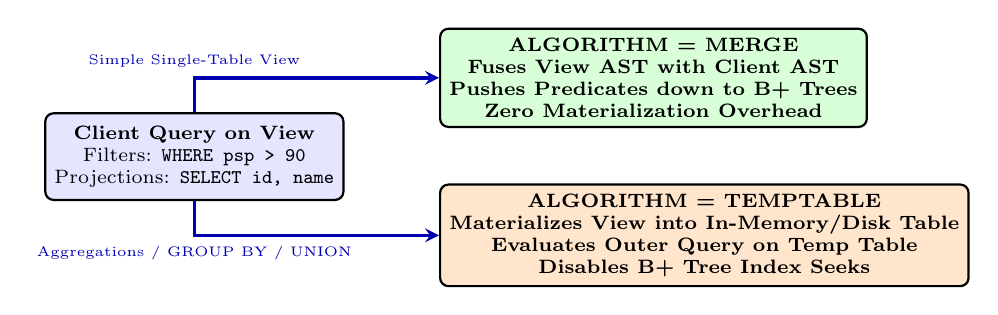
\begin{tikzpicture}[
    box/.style={draw, rectangle, rounded corners=3pt, thick, align=center, fill=blue!10, minimum width=3.0cm, minimum height=1.1cm, font=\scriptsize},
    mergebox/.style={draw, rectangle, rounded corners=3pt, thick, align=center, fill=green!15, minimum width=3.4cm, minimum height=1.1cm, font=\scriptsize\bfseries},
    temptable/.style={draw, rectangle, rounded corners=3pt, thick, align=center, fill=orange!20, minimum width=3.4cm, minimum height=1.1cm, font=\scriptsize\bfseries},
    arr/.style={->, >=stealth, very thick, color=blue!70!black}
]
    \node[box] (query) {\textbf{Client Query on View}\\Filters: \texttt{WHERE psp > 90}\\Projections: \texttt{SELECT id, name}};
    \node[mergebox, right=1.2cm of query, yshift=1.0cm] (merge) {\textbf{ALGORITHM = MERGE}\\Fuses View AST with Client AST\\Pushes Predicates down to B+ Trees\\Zero Materialization Overhead};
    \node[temptable, right=1.2cm of query, yshift=-1.0cm] (temp) {\textbf{ALGORITHM = TEMPTABLE}\\Materializes View into In-Memory/Disk Table\\Evaluates Outer Query on Temp Table\\Disables B+ Tree Index Seeks};
    
    \draw[arr] (query) |- node[above, font=\tiny] {Simple Single-Table View} (merge);
    \draw[arr] (query) |- node[below, font=\tiny] {Aggregations / GROUP BY / UNION} (temp);
\end{tikzpicture}
\caption{Relational View Execution Strategies in MySQL: AST Merging vs. Temporary Table Materialization. View merging fuses client predicates directly into the underlying B+ Tree scans, whereas temporary table materialization computes the full view before evaluating outer filters.}
\label{fig:views}
\end{figure*}

\begin{enumerate}
    \item \textbf{\texttt{ALGORITHM = MERGE}}: The query optimizer unpacks the view definition and merges its \texttt{WHERE} clauses, joins, and projections directly into the referencing query's Abstract Syntax Tree.
    \begin{itemize}
        \item Predicate pushdown operates across the combined query, allowing outer filters (\texttt{WHERE psp > 90}) to utilize the base table's B+ Tree indexes directly.
        \item Memory overhead is negligible ($\mathcal{O}(1)$).
    \end{itemize}
    \item \textbf{\texttt{ALGORITHM = TEMPTABLE}}: When a view contains non-mergeable constructs (such as \texttt{GROUP BY}, aggregate functions, \texttt{DISTINCT}, \texttt{HAVING}, \texttt{UNION}, or window functions), the engine cannot fuse the ASTs.
    \begin{itemize}
        \item The engine materializes the entire view into an internal in-memory or on-disk temporary table.
        \item The outer query then scans this temporary table. Outer filters cannot be pushed down into base table indexes, dramatically increasing query latency.
    \end{itemize}
\end{enumerate}

\subsection{View Updatability and Determinism}
A common enterprise requirement is executing Data Manipulation Language mutations (\texttt{INSERT}, \texttt{UPDATE}, \texttt{DELETE}) through view interfaces.
\begin{theorem}[View Updatability Invariant]
A relational view is updatable if and only if there exists an injective (one-to-one) deterministic mapping between each row in the view and exactly one physical tuple in an underlying base table.
\end{theorem}
Consequently, views that contain the following operations are strictly **read-only**:
\begin{itemize}
    \item Aggregate reduction functions (\texttt{SUM}, \texttt{COUNT}, \texttt{AVG}, etc.).
    \item Relational grouping (\texttt{GROUP BY}) and post-filtering (\texttt{HAVING}).
    \item Deduplication operators (\texttt{DISTINCT}).
    \item Set operations (\texttt{UNION}, \texttt{INTERSECT}, \texttt{EXCEPT}).
    \item Multi-table joins where the update target is not an unambiguous key-preserved table.
\end{itemize}

% -----------------------------------------------------------------------------
\section{The Comprehensive SQL DQL Logical Query Lifecycle}
\label{sec:execution_order}

The complete logical execution lifecycle of a complex relational query containing subqueries and views formalizes why clauses behave as observed:

\begin{table*}[htbp]
\caption{Comprehensive SQL DQL Logical Query Execution Pipeline with Nested Subqueries and Views}
\label{tab:execution_pipeline}
\centering
\scriptsize
\begin{tabular}{cp{3.2cm}p{3.8cm}p{7.2cm}}
\toprule
\textbf{Step} & \textbf{SQL Processing Phase} & \textbf{Relational Operation} & \textbf{Subquery / View Resolution Mechanism} \\
\midrule
1 & \textbf{\texttt{VIEW EXPANSION}} & Query Tree Rewriting & Unpacks views; fuses AST via \texttt{MERGE} or schedules \texttt{TEMPTABLE} materialization. \\
2 & \textbf{\texttt{FROM / JOIN}} & Base Cartesian Product / Joins & Materializes derived tables; executes join algorithms (INLJ, Hash Join, Sort-Merge). \\
3 & \textbf{\texttt{ON}} & Join Predicate Evaluation & Evaluates join predicates; governs outer join preservation. \\
4 & \textbf{\texttt{WHERE}} & Tuple Selection ($\sigma$) & \textbf{Executes scalar, \texttt{IN}, \texttt{ALL}, \texttt{ANY}, and \texttt{EXISTS} subqueries; applies SARGable index seeks.} \\
5 & \textbf{\texttt{GROUP BY}} & Equivalence Partitioning & Groups tuples into equivalence buckets; collates NULLs into single group. \\
6 & \textbf{AGGREGATION} & Multi-Set Reduction ($f$) & Computes \texttt{COUNT}, \texttt{SUM}, \texttt{AVG}, \texttt{MIN}, \texttt{MAX}; eliminates NULL values. \\
7 & \textbf{\texttt{HAVING}} & Group Selection ($\sigma_{\text{group}}$) & \textbf{Evaluates group-level subqueries and aggregate thresholds post-aggregation.} \\
8 & \textbf{\texttt{SELECT}} & Projection ($\pi$) \& Expressions & Evaluates scalar subqueries in projection list; formats aliases and string concatenations. \\
9 & \textbf{\texttt{DISTINCT}} & Duplicate Tuple Suppression & Deduplicates tuples via streaming B+ Tree scans or in-memory hash sets. \\
10 & \textbf{\texttt{ORDER BY}} & Physical Sequence Ordering & Filesort buffer allocation; multi-column deterministic tie-breaking. \\
11 & \textbf{\texttt{LIMIT / OFFSET}} & Stream Windowing & Discards offset records; emits final output window. \\
\bottomrule
\end{tabular}
\end{table*}

Understanding this lifecycle explains why:
\begin{enumerate}
    \item Derived tables in \texttt{FROM} (Step 2) are evaluated before \texttt{WHERE} (Step 4), allowing derived aggregates to act as static filters for the outer query.
    \item Correlated subqueries in \texttt{WHERE} (Step 4) are invoked once per surviving outer tuple, whereas decorrelated joins execute once at Step 2.
    \item Aliases created in \texttt{SELECT} (Step 8) cannot be referenced in \texttt{WHERE} (Step 4) or \texttt{GROUP BY} (Step 5).
\end{enumerate}

% -----------------------------------------------------------------------------
\section{Conclusion and Enterprise Engineering Blueprint}
\label{sec:conclusion}

Relational subqueries and virtual views represent foundational abstractions for modular, secure, and expressive query engineering. This research paper has formalized the core mechanics governing subqueries, quantified comparisons, and view pipelines:

\begin{enumerate}
    \item \textbf{Enforce Scalar Subquery Determinism}: Guard scalar subqueries with unique indexed keys or aggregate reduction functions (\texttt{MAX}, \texttt{MIN}) to eliminate runtime Error 1242 cardinality violations.
    \item \textbf{Mandate Derived Table Aliases}: Always assign explicit aliases to table expressions in the \texttt{FROM} clause to satisfy ANSI SQL data dictionary requirements.
    \item \textbf{Resolve Nested Aggregates via Derived Tables}: Never attempt direct aggregate nesting (\texttt{MIN(AVG())}); encapsulate the inner grouping in a derived table and compute outer summaries over the materialized result.
    \item \textbf{Prefer NOT EXISTS over NOT IN}: Always deploy \texttt{NOT EXISTS} for negative set filtering to guarantee complete immunity against the fatal Three-Valued Logic NULL contamination trap.
    \item \textbf{Beware of Vacuous Truth in ALL}: Remember that universal quantification against an empty subquery ($x > \text{ALL}(\emptyset)$) evaluates vacuously to \texttt{TRUE}.
    \item \textbf{Deploy ANY for Quantified Inequalities}: Use \texttt{ANY} when testing relational inequalities ($>, <, \ge, \le$) against multi-row columnar subqueries, as \texttt{IN} is restricted strictly to equality comparisons.
    \item \textbf{Decorrelate Quadratic Loops}: Refactor correlated subqueries into explicit derived table joins to reduce execution latency from $\mathcal{O}(N \cdot M)$ to $\mathcal{O}(N + M)$.
    \item \textbf{Design Views for AST Merging}: Maintain simple, unaggregated view definitions where possible to allow the query planner to deploy \texttt{ALGORITHM = MERGE}, preserving B+ Tree index range seeks.
    \item \textbf{Isolate Sensitive Data via Views}: Restrict application database credentials to virtual views with masked columns and row-level tenant filters, revoking direct base table permissions.
    \item \textbf{Respect View Updatability Boundaries}: Never issue \texttt{UPDATE} or \texttt{INSERT} statements through views that contain aggregations, \texttt{GROUP BY}, or \texttt{DISTINCT}.
\end{enumerate}

By adhering to this architectural blueprint, database engineers and software architects guarantee deterministic query correctness, bounded computational complexity, and secure multi-tenant data isolation across high-scale enterprise systems.

% -----------------------------------------------------------------------------
\begin{thebibliography}{10}
\setlength{\itemsep}{1pt}

\bibitem{codd1970}
E.~F.~Codd, ``A Relational Model of Data for Large Shared Data Banks,'' \emph{Communications of the ACM}, vol.~13, no.~6, pp.~377--387, 1970.

\bibitem{date2004}
C.~J.~Date, \emph{Database in Depth: Relational Theory for Practitioners}.\hskip 1em plus 0.5em minus 0.4em\relax Sebastopol, CA: O'Reilly Media, 2005.

\bibitem{sql6notes}
Scaler Academy, ``SQL Class 6: Subqueries, Correlated Subqueries, Quantified Comparisons, and Relational Views,'' Technical Lecture Notes (Note 22 Dec 2025), Nov.~2026.

\bibitem{mysql84}
Oracle Corporation, ``MySQL 8.4 Reference Manual: Subqueries, Derived Tables, and Views Optimization,'' Oracle Technology Network, 2024. [Online]. Available: \url{https://dev.mysql.com/doc/refman/8.4/en/subqueries.html}

\bibitem{selinger1979}
P.~G.~Selinger, M.~M.~Astrahan, D.~D.~Chamberlin, R.~A.~Lorie, and T.~G.~Price, ``Access Path Selection in a Relational Database Management System,'' in \emph{Proceedings of the 1979 ACM SIGMOD International Conference on Management of Data}, pp.~23--34, 1979.

\bibitem{gray1993}
J.~Gray and A.~Reuter, \emph{Transaction Processing: Concepts and Techniques}.\hskip 1em plus 0.5em minus 0.4em\relax San Mateo, CA: Morgan Kaufmann Publishers, 1993.

\end{thebibliography}


\end{document}
